%Definujte klíčové faktory a rizika využití BYOD v bankovním prostředí.

\section{Trendy v ICT pro spotřebitele}\label{trendy} \todo{nejake statistiky a magic quadranty}

Podle ředitele odboru statistik a rozvoje Českého statistického úřadu Martina Mana \textit{Je zajímavé, že počet uživatelů internetu převyšuje počet uživatelů počítače. Je to dáno hlavně rozmachem chytrých telefonů a jiných přenosných zařízení, která jsou častěji využívána i k přístupu na internet. Lze předpokládat, že internet se ve spojení s mobilem brzy stane široce rozšířenou technologií používanou napříč všemi věkovými a vzdělanostními  kategoriemi,} \todo{citace https://www.czso.cz/csu/czso/chytre-telefony-zvysuji-pocet-uzivatelu-internetu}. Podle předsedkyně Českého statistického úřadu Ivy Ritschelové v citátu z května 2016 \textit{Až do roku 2013 dominovaly českým domácnostem klasické stolní počítače. Vloni je vystřídaly počítače přenosné. Mělo je 55 \% všech domácností, resp. 75 \% domácností, které jsou vybaveny počítačem}.

Podle výzkumu provedeným společností TNS Infratest pro společnost Google vlastnilo v roce 2016 v České republice chytrý telefon připojený k internetu 50 \% všech obyvatel. \todo{https://www.consumerbarometer.com/en/about/}  To je oproti 17 \% z roku 2012 drastický nárůst a je možné pozorovat dále vzrůstající trend \ref{uzivateleSmartphone}. Dále zřejmé, že trend v České republice bude dále dohánět rozšíření chytrých mobilních telefonů v technologicky vyspělejších zemích jako jsou Spojené státy, nebo sousední Německo. Ve Spojených státech dosáhla adopce chytrých mobilních v roce 2016 72 \%.

\begin{figure}[h!]\label{uzivateleSmartphone}
\centering
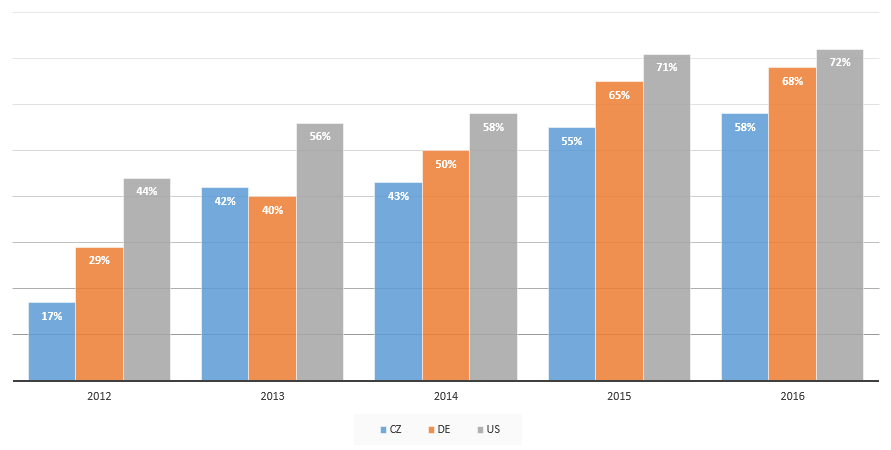
\includegraphics[width=13cm]{img/uzivateleSmartphone}
\caption{Poměrná část uživatelů chytrých telefonů k celé populaci v České republice, Německu a spojených státech. Zdroj: } 
\end{figure}\todo{citovat }

Jiným typem zařízení, které zaznamenávají zvýšenou popularity jsou tablety. V roce 2012 vlastnilo v České republice tablet připojený k internetu 4 \% obyvatelstva. V roce 2016 to bylo již 26 \% což je více než šestinásobek uživatelů v rozmezí ctyř let. V USA vlastní tablet připojený k internetu dokonce 42 \% obyvatelstva a trend je nadále stoupající. 

\begin{figure}[h!]\label{uzivateleTablet}
\centering
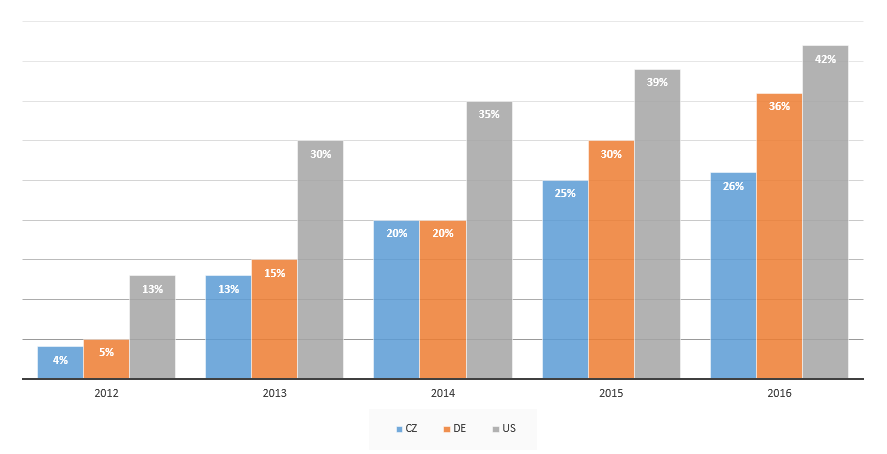
\includegraphics[width=13cm]{img/uzivateleTablet}
\caption{Poměrná část uživatelů tabletů k celé populaci v České republice, Německu a spojených státech. Zdroj: } 
\end{figure}\todo{citovat }

Další zajímavou statistikou je průměrný počet zařízení připojených k síti internet na jednoho obyvatele daného státu v daném státě. V roce 2012 obyvatel České republiky vlastnil v průměru 1,6 zařízení, zatímco v roce 2016 to bylo 2,5. Průměrný Američan vlastnil v roce 2016 3.5 zařízení připojených k internetu. To znamená nejspíše počítač, chytrý telefon, tablet a další zařízení.

\begin{figure}[h!]\label{pocetZarizeni}
\centering
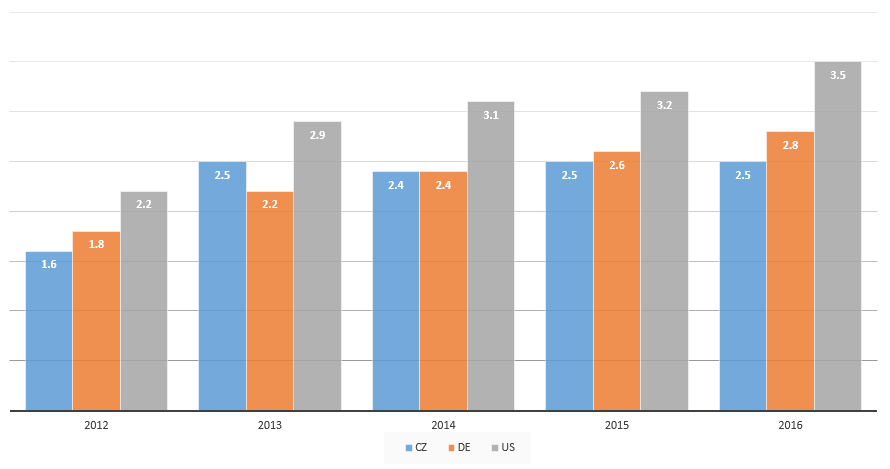
\includegraphics[width=13cm]{img/pocetZarizeni}
\caption{Průměrný počet zařízení připojených k internetu na obyvatele v České republice, Německu a Spojených státech. Zdroj: } 
\end{figure}\todo{citovat }

Tato čísla ukazují, že počet obyvatel vlastnících zařízení z oblasti informačních a komunikačních technologií v posledních letech dramaticky roste. Lidé vlastnící své soukromé zařízení si vytvářejí návyky a začínají upřednostňovat některé technologie nad jinými.

Své návyky s obsluhou ICT ve svém soukromém životě by tak někteří zaměstnanci rádi začali uplatňovat i v životě pracovním. To může přinést jak zaměstnanci tak zaměstnavateli mnohé výhody, ale zároveň mnohá úskalí, se kterými je třeba se vyrovnat. Nastolená praxe, kdy zaměstnanec používá své vlastní zařízení k pracovním účelům, se souhrnně označuje termínem BYOD.



\section{Charakteristika BYOD}

BYOD je zkratka v anglickém jazyce znamenající "Bring your own device". Oxfordský slovník jej vysvětluje jako postup vedoucí k umožnění zaměstnancům organizace používat jejich vlastní počítače, chytré telefony a další zařízení k pracovním účelům. \todo{https://en.oxforddictionaries.com/definition/BYOD} 

Slovník Cambridge definuje BYOD jako postup firem nebo škol, který říká, že zaměstnanci nebo studenti si mohou přinést své vlastní počítače, telefony, atd.  do práce nebo školy za účelem jejich využití k práci. \todo{citace http://dictionary.cambridge.org/dictionary/english/byod}

Poradenská společnost Gartner BYOD definuje jako \textit{alternativní strategii povolující zaměstnancům, obchodním partnerům a dalším uživatelům používání osobně zvolených a zakoupených koncových zařízení ke spouštění podnikových aplikací a přístupu k datům. To typicky znamená chytré telefony a tablety, ale tato strategie může být také použita pro osobní počítače. Může obsahovat i finanční kompenzace.}

Konzultační společnost Deloitte definuje BYOD jako použití zařízení vlastněných zaměstnancem pro přístup k přístupu k podnikovému obsahu nebo sítím. \todo{citace https://www2.deloitte.com/content/dam/Deloitte/uk/Documents/about-deloitte/deloitte-uk-understanding-the-bring-your-own-device\%20landscape.pdf} Dále dále upřesňuje ve třech kategoriích a to zařízení, schopnosti a charakteristika. 

Zařízeníje specifikované jako vybavené procesorem a to specificky chytré telefony, tablety nebo počítače. Schopnosti se mohou lišit od pouhého přístupu k internetu skrze firemní síť po přístup k podnikovým aplikacím a systémům. Charakteristiou BYOD může být používání vlastních zařízení jako doplněk k firemním zařízením, jako náhradu firemního zařízení, nebo povolení k užití zařízení, které firma není zaměstnanci ochotna zajistit vlastními zdroji. 

Podle dat ze služby Google Analytics \todo{citace} se výraz BYOD začal rozšiřovat začátkem roku 2012. Graf \ref{hledaniBYOD} ukazuje popularitu vyhledávání výrazu BYOD za použití vyhledávače Google v čase vztažené relativně k období, kdy byl zadaný výraz vyhledáván nejčastěji. Je zřejmé, že zájem o tuto problematiku nepolevuje.

\begin{figure}[h!]\label{hledaniBYOD}
\centering
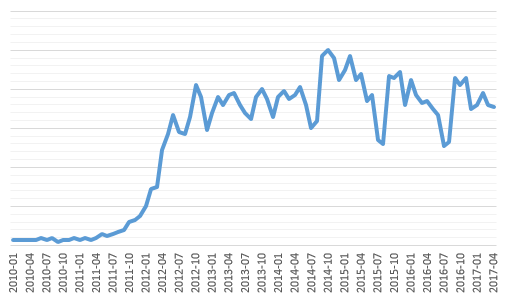
\includegraphics[width=13cm]{img/hledaniBYOD}
\caption{Relativní popularita vyhledávání termínu BYOD vztažená k maximální popularitě v daném období podle Google Analytics Zdroj: www.analytics.google.com } 
\end{figure}\todo{citovat }
 

Článek \todo{citovat consumeration} zmiňuje mnohé výhody modelu, kdy zaměstnanci používají svá vlastní zařízení jako například zvýšenou flexibilitu a produktivitu zaměstnanců. Dále zmiňuje snížení nákladů na technickou podporu zařízení, jelikož za svá zařízení si zaměstnanci odpovídají sami.

Na druhou stranu článek zmiňuje nutnost zavedení omezujících pravidel, jelikož nefiremní zařízení s sebou přinášejí řadu hrozeb jako jsou úniky dat či napadení firemní infrastruktury škodlivým software.  Další zmíněné negativum osobních zařízení ve firemním prostředí je nebezpečí využívání pracovní doby k soukromým účelům jako je hraní her, streamování videí a dalším činnostem snižujícím pracovní morálku.

Vzhledem k masovému rozšíření informačních technologií mezi spotřebiteli se stává pro firmy nutností zaujmout k soukromým zařízením jednoznačný postoj. BYOD zařízení ve firemním již nejsou pouze možností, ale každodenní realitou.

V době, kdy mnozí zaměstnanci vlastní výkonné chytré telefony, tablety, či dokonce nositelnosti a vnášejí je do firemního prostředí je nutné nastavit jasná pravidla, aby byla chráněna firemní infrastruktura a data.

Podle Pavla Housera z Hospodářských novin \todo{citovat http://ictrevue.ihned.cz/c3-65260640-0ICT00\_d-65260640-byod-prinasi-firmam-vyssi-produktivitu-i-bezpecnostni-rizika} již BYOD do firem prorostlo a stalo se realitou i přes snahu některých firem o zákaz. Autor tvrdí, že na konceptu BYOD vydělaly především firmy, které jej pochopily nejen jako hrozbu, ale i příležitost. 

Naopak podle tiskové zprávy společnosti Intel publikované v Hospodářských novinách \todo{ citace http://ictrevue.ihned.cz/c3-65456950-0ICT00\_d-65456950-byod-po-cesku-pouze-v-7-firem-vita-vyuziti-soukromych-pocitacu-zamestnancu} vítá koncept BYOD pouze 7 \% českých firem, zbytek se k tématu staví odměřeně. Respondenti jejího průzkumu mají výhrady především k bezpečnosti, viz \ref{intelBYOD}.

\begin{figure}[h!]\label{intelBYOD}
\centering
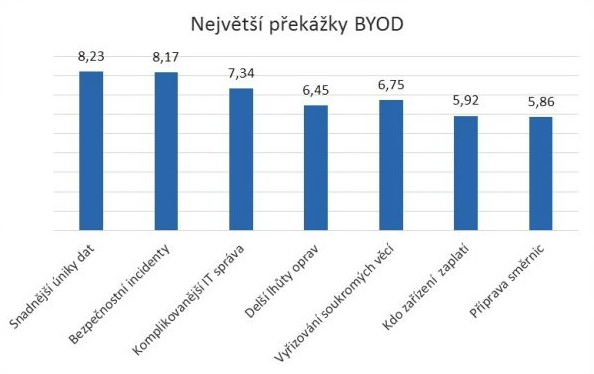
\includegraphics[width=12cm]{img/intelBYOD}
\caption{Největší negativa BYOD podle průzkumu společnosti Intel ohodnocené ve škále 1 až 10. Zdroj: } 
\end{figure}\todo{citovat http://ictrevue.ihned.cz/c3-65456950-0ICT00\_d-65456950-byod-po-cesku-pouze-v-7-firem-vita-vyuziti-soukromych-pocitacu-zamestnancu }

Společnost Deloitte ve svém článku uvádí tři možné přístupy k BYOD. Tolerovaní, zákaz nebo řízený BYOD program. Zatímco zákaz s sebou nese vysoké riziko nerespektování zaměstnanci a tím pádem i riziko bezpečnostní, řízený BYOD s sebou nese náklady na přípravu, zaškolení a provoz.

Jako hlavní výhody uvádí:
\begin{itemize}
\item Snížení nákladů na IT
\item Zvýšení produktivity
\item Zvýšení spokojenosti zaměstnanců
\item Lepší porozumění zákazníkům
\item Lepší operační flexibilita
\end{itemize}

Snížení nákladů tkví především v podpoře. Zaměstnanci si musí vyřešit problémy se svým hardware na vlastní náklady. Dále je uvedeno, že zaměstnanci mají tendenci si pořizovat výkonnější zařízení, než by jim poskytla jejich firma. 

Zvýšením produktivity se projevuje zvýšením ochoty pracovat mimo pracovní dobu, zvýšení efektivity práce vzhledem k práci se známým zařízením a v neposlední řadně užíváním moderních technologií, které by jinak nemuseli být pro zaměstnance dostupné. 

Spokojenost zaměstnanců je zvýšená díky tomu, že si mohou vybrat zařízení, které jim nejlépe vyhovuje. Porozuměním zákázníkům je myšleno přiblížení zákazníkům díky šírší paletě zařízení používaných ve firmě a tím pádem lepšímu pochopení jakým způsobem mohou zákazníci pracovat s veřejnými aplikacemi. Zaměstnanci s nejmodernějšími technologii také vylepšují obraz firmy.

Zvýšená operační flexibilita se projevuje u jednoduššího náboru a zaškolování nových zaměstnanců, jednodušší začleňování zaměstnanců z firem po akvizicích, jednodušší práce s kontraktory a dále je to možnost práce z domu.


Podle studie \todo{https://pdfs.semanticscholar.org/9ffd/5c3d0511c8841f9bbe6b38b1e542dea13da7.pdf} trend užívání spotřebních zařízení a aplikací k pracovním účelům způsobuje střety zájmů s IT oddělením. Jedná se o střet z hlediska cílů, střet chování a střet identity. Zatím co cílem IT oddělení je zařízení kontrolovat, zaměstnanci a jejich vlastní zařízení jim to ztěžují. Zaměstnanci i s vlastními zařízeními předpokládají, že IT oddělení jim bude schopné pomoci řešit jejich problémy, ale to bohužel v případě použití nestandardních zařízení a postupů není možné. Konflikt identity znamená jev, kdy role IT oddělení se s příchodem BYOD mění, avšak zaměstnanci IT oddělení mají problémy novou roli uchopit.

\section{Aspekty BYOD politiky}

Pro úspěšné nasazení BYOD programu do firmy je nezbytně nutné nastavit jasná pravidla.

Společnost Deloitte doporučuje věnovat se následujícím aspektům \todo{citace }:
\begin{itemize}
\item Způsobilost zaměstnanců
\item Příspěvky na BYOD
\item Model podpory pro soukromá zařízení zaměstnanců
\item Školení zaměstnanců a řízení změn
\item Soukromí a legislativa
\end{itemize}

Ne všechny pracovní úkony je možné provádět na nefiremních zařízení, proto je třeba určit pro které zaměstnance je BYOD program vhodný. 
Je vhodné zvážit zda a jakým způsobem přispívat zaměstnancům na jejich zařízení používaná k práci. Způsob dotace by měl být co nejjednodušší. Také je třeba nastavit mechanismus pro řečení problémů. Osvědčila se různá komunitní fóra a dsikuzní skupiny, avšak pro komplexnější problémy může být třeba konzultace se specialistou. Dále je třeba skloubit používání soukromých zařízení s firemními politikami. Je třeba seznámit zaměstnance s bezpečnostními riziky, která z BYOD plynou. 

Požadavky na zabezpečení firemních dat často mohou být v rozporu požadavků zaměstnanců na jejich soukromí. Jedná se například o požadavek zaměstnavatele mít možnost vzdáleně vymazat data ze zařízení po jeho odchodu z firmy, na druhou stranu zaměstnanec nemá zájem na tom, aby zaměstnavatel měl přístup k jeho soukromým datům nebo monitoroval jeho aktivity.

\section{Právní prostředí v ČR}

Právními aspekty BYOD v prostředí českých společností se zabývá analýza advokátů kanceláře Havel, Holásek \& Partners z ledna 2017 \todo{citace }. Český právo BYOD přímo neupravuje a proto je třeba vycházet z ustanovení zákoníku práce. Podle § 2 zákoníku práce je \textit{zaměstnavatel povinen vytvářet zaměstnanci podmínky pro plnění pracovních úkonů a poskytnout mu k tomu pracovní pomůcky.}

Zákon umožňuje zaměstnanci taktéž použít pomůcky vlastní, ale musí to být dobrovolné rozhodnutí na základě dohody se zaměstnavatelem. Zároveň podle § 190 odst. 1  zákoníku práce, musí být zaměstnanci poskytnuta kompenzace za opotřebení.

Dalším zjištěním analýzy je, že pokud zaměstnanec odmítne využívat BYOD, musí mu zaměstnavatel nabídnout jiné řešení. Pokud by se tak nestalo, \textit{zaměstnanec bys se mohl odvolat na nemožnost vykonávat práci pro překážku na straně zaměstnavatele ve smyslu § 208 zákoníku práce a požadovat náhradu mzdy/platu ve výši průměrného výdělku.}

Dohoda se zaměstnancem může být ve formě dodatku k pracovní smlouvě nebo smlouvou samostatnou. Nesmí vést k rozdílnému zacházení k zaměstnancům, kteří do BYOD programu nevstoupili. Kompenzace musí být odlišena od firemních bonusů a mzdy, výše však není stanovena. 

Analýza \todo{zase citnout} doporučuje vydání interní směrnice, která stanoví práva a povinnosti zaměstnance. Je třeba vzít v potaz, že směrnice nesmí zaměstnanci ukládat povinnosti nad rámec zákona, a proto je některé záležitosti lepší upravovat přímo v dohodě se zaměstnancem.

V době psaní této práce probíhá v parlamentu ČR legislativní proces novelizace zákona č. 262/2006 Sb. jako sněmovní tisk č. 903/0 \todo{ citovat http://www.psp.cz/sqw/historie.sqw?o=7\&t=903\&snzp=1}, který se problematiky BYOD taktéž může dotknout.

Podle Pavla Marce z Advokátní kanceláře Novalia \todo{citace http://www.e15.cz/finexpert/vydelavame/rady-jak-vyzrat-na-home-office-chystana-regulace-viri-nejvetsi-emoce-1330808} novela zákona předjímá a tím pádem legalizuje BYOD. Doporučuje platit zaměstnancům měsíční nezdanitelné paušály jako kompenzaci za BYOD, tak zároveň jako kompenzaci nákladů v režimu tzv. "home office". Autor tvrdí, že forma paušálu usnadní administrativu, je osvobozený od daně, ale přitom snižuje daňový základ. 

\section{BYOD z hlediska bezpečnosti}

V roce 2016 provedla společnost Ponemon Institute průzkum mezi 694 odborníky na IT a IT bezpečnost ve Spojených státech. \todo{citovat ponemon https://cdn2.hubspot.net/hubfs/150964/2016\_State\_of\_Endpoint\_Report.pdf}. Zaměřuje se na hodnocení rizik spojených s koncovými zařízeními v IT jako jsou servery, desktopy, mobilní zařízení a další. 76 procent účastníků si myslí, že v roce 2016 stoupla závažnost malwarových útoků. Zároveň 56 procent dotázaných si myslí, že útoky jsou lépe skryté a tedy mnohem náročnější na detekci. I proto je čím dál náročnejší strážit firemní data.


\subsection{Trendy v IT bezpečnosti}

Studie odhalila několik trendů v oblasti IT bezpečnosti. Kybernetické útoky využívají stále více destruktivního malware jako jsou Cryptolocker nebo Shamoon. Pouze 38 dotázaných odborníků má ve své firmě připravenou strategii pro boj proti destruktivnímu malware.

Největším rizikem v IT bezpečnosti dále zůstávají uživatelé a jejich zařízení ignorující bezpečnostní politiky firmy. Hrozba způsobená nezabezpečenými mobilními zařízeními stoupla podle 50 procent dotázaných. Nejvíce škody podle průzkumu momentálně způsobují útoky typu zero-day. Dále jsou to útoky typu denial of service.

\begin{figure}[h!]\label{hrozby}
\centering
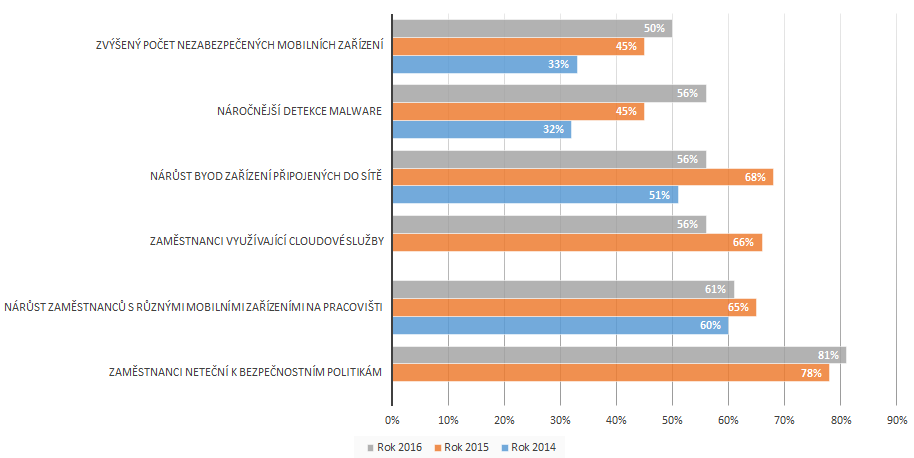
\includegraphics[width=14cm]{img/hrozby}
\caption{Jaké jsou největší hrozby pro bezpečnost koncových zařízení v organizacích účastníků průzkumu? Zdroj: } 
\end{figure}\todo{citovat }

Až 80 procent respondentů si myslí, že mobilní zařízení v jejich firmě byla během posledních dvanácti měsíců cílem útoku malware. Největší hrozbou jsou přenosné počítače a chytré telefony. Velkým rizikem je užívání komerčních cloudových aplikací uživateli a BYOD. Většina odborníků si myslí, že rozpočet pro zajištění IT bezpečnosti není dostatečný. 

\begin{figure}[h!]\label{hrozbyUtoky}
\centering
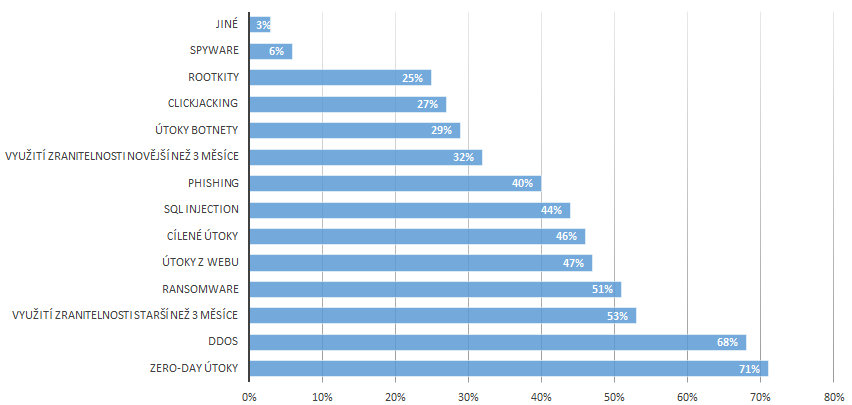
\includegraphics[width=14cm]{img/hrozbyUtoky}
\caption{Jaká část účastníků průzkumu si myslí, že daný typ útoku způsobuje ty nejzávažnější incidenty? Zdroj: } 
\end{figure}\todo{citovat }

Zabezpečení koncových zařízení však hraje v bezpečnostní strategii IT čím dál větší roli. Oraganizace se plánují více soustředit na detekci a reakci, než na prevenci. 





\begin{figure}[h!]\label{hrozbyZarizeni}
\centering
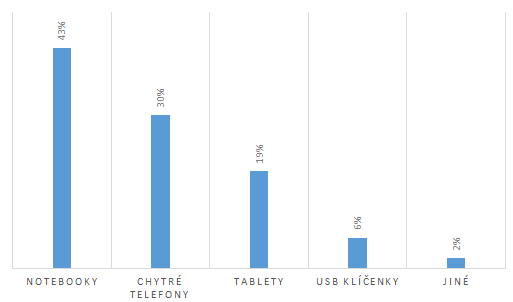
\includegraphics[width=12cm]{img/hrozbyZarizeni}
\caption{Jak velká část účastníků průzkumu si myslí, že největší hrozbou pro organizaci je právě daný typ zařízení? Zdroj: } 
\end{figure}\todo{citovat }



\begin{figure}[h!]\label{hrozbyDuvody}
\centering
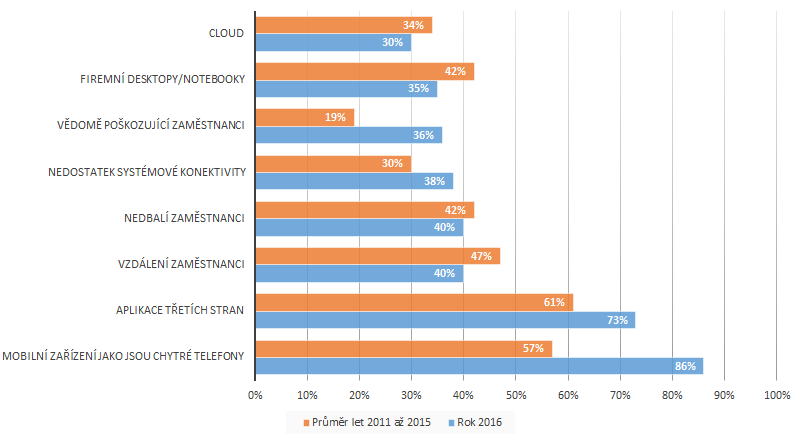
\includegraphics[width=13cm]{img/hrozbyDuvody}
\caption{Jaká část účastníků průzkumu očekává nejvyšší nárůst potencionálního rizika pro bezpečnost IT v daných kategoriích? Zdroj: } 
\end{figure}\todo{citovat }





\section{Specifika bankovního prostředí}
\todo{jak je regulovan banking a ICT v bankingu}